% ======== Template para elaboracion de informes ========
% version: 1.3  - Jul/12 
% autor: www.fing.edu.uy/~jperez 
% =======================================================
%
% ----- LICENCIA -----
% Este trabajo es distribuido bajo la licencia LaTeX Project Public License
% Puede y DEBE ser usado, modificado y distribuido gratuitamente.
%
% This work is distributed under the LaTeX Project Public License (LPPL)
% ( http://www.latex-project.org/ ). Must and may be freely used,
% distributed and modified.
% ---------------------
%
%
% ----- INSTRUCCIONES -----
% ver readme
% compilacion:  PdfLaTeX
%
% **************************************************************************
\documentclass[a4paper,11pt]{article}

% ===== Algunos paquetes a ser usados =====

% para poder escribir con tildes
\usepackage[T1]{fontenc}
\usepackage[utf8]{inputenc}
\usepackage[spanish]{babel}
\usepackage{enumitem}
% fuentes para escribir símbolos
\usepackage{amsfonts}
\usepackage{amssymb}
\usepackage{amsthm}
\usepackage{mathrsfs}
%Geometria
\usepackage[a4,  margin=2in]{geometry}

% inclusión de graficos
\usepackage{graphicx}

\usepackage{hyperref}
\pagestyle{empty}
\usepackage[centertags]{amsmath}
% ====================================

%===PASCAL===
\usepackage{listings}             % Include the listings-package
\lstset{language=Pascal}

%==para tablas===
\usepackage{tabu}
% ===== Encabezado =====
\pagestyle{myheadings}
\markright{Germán Faller  \& Octavio Perez Kempner \hfill MOR - }
% ======================


% ===== Ajuste layout pagina =====
%\usepackage{fullpage}
\oddsidemargin=-.25cm
\setlength{\textwidth}{160mm}
\setlength{\textheight}{210mm}
\addtolength{\voffset}{-5pt}
% ================================
% ===LOGICA DERIVACIONES ====
\usepackage{proof}
\usepackage[utf8]{inputenc}
\usepackage{tex/macros}
%%\usepackage{../../../tex/proof}
\usepackage{lscape}
%\usepackage[notodo]{../../../tex/notasDoc}
%\usepackage[inline]{../../../tex/notasDoc}
\usepackage{graphicx}

\renewcommand{\mlforall}[2]{\ensuremath{\bar\forall #1,\ #2}}
\renewcommand{\mlexists}[2]{\ensuremath{\bar\exists #1,\ #2}}
\newcommand*{\Scale}[2][4]{\scalebox{#1}{$#2$}}%

\usepackage{geometry}
\geometry{
	a4paper,
	total={170mm,257mm},
	left=15mm,
	top=20mm,
}

\usepackage{rotating}

% =================================

% --- commandos ---
\newcommand{\ds}{\displaystyle}
\def\x{{\bf x}}
% -----------------
% ===Funciones Booleanas ====
\usepackage{pst-all}
\usepackage{fancybox}
\newcommand{\mystar}{{\fontfamily{lmr}\selectfont$\star$}}
\def\R{{\mathbb R}} 
\def\N{{\mathbb N}}
\def\F{{\mathbb F}} 
\def\BF{\ensuremath{\mathcal{BF}}} %% Boolean functions set
\mathchardef\mslash="202F
\newtheorem{obs}{\scshape{Observación}}[section]
\newtheorem{demo}{\scshape{Demostración}}
\newtheoremstyle{break}
{\topsep}{\topsep}%
{\itshape}{}%
{\bfseries}{}%
{\newline}{}%
\theoremstyle{break}
\newtheorem{defi}{\scshape{Definición}}[section]
% ========  Aca comienza el cuerpo del texto ==========
\title{Metaheurísticas y Optimización Sobre Redes \\ Obligatorio 2017}
\author{Germán Faller  \& Octavio Perez Kempner\\ Instituto de Computación\\ Facultad de Ingeniería}
\date{v1.0}

\begin{document}

% hace título
\maketitle

%hace índice
\tableofcontents

\newpage

\section{Introducción}

El obligatorio a resolver consiste en abordar el problema de diseñar una red de Trenes Ligeros (Light Rail Transit o LRT) para Montevideo.

Considerando como característico de nuestra capital el tener una población que tiende a vivir lejos de su centro de estudio y/o trabajo se supondrá que en la ciudad existen tres puntos de concentración: Tres Cruces, Plaza Independencia y el Palacio Municipal que serán los destinos de los pasajeros en la mañana y su punto de partida en la tarde. Se asumirá que al llegar al cualquiera de estos puntos la movilidad urbana entre ellos será rápida y contará con la infraestructura adecuada.

Por otra parte al identificar cuatro agregadores zonales, las terminales: Cerro, Colón, Carrasco y Pocitos se tendrá como objetivo de la red LRT definir los caminos desde cualquier agregador zonal a cualquier punto de concentración.

A Continuación se muestran las terminales, los puntos de concentración y las posibilidades de los tramos a seleccionar para construir la red LRT.
\begin{align*}
	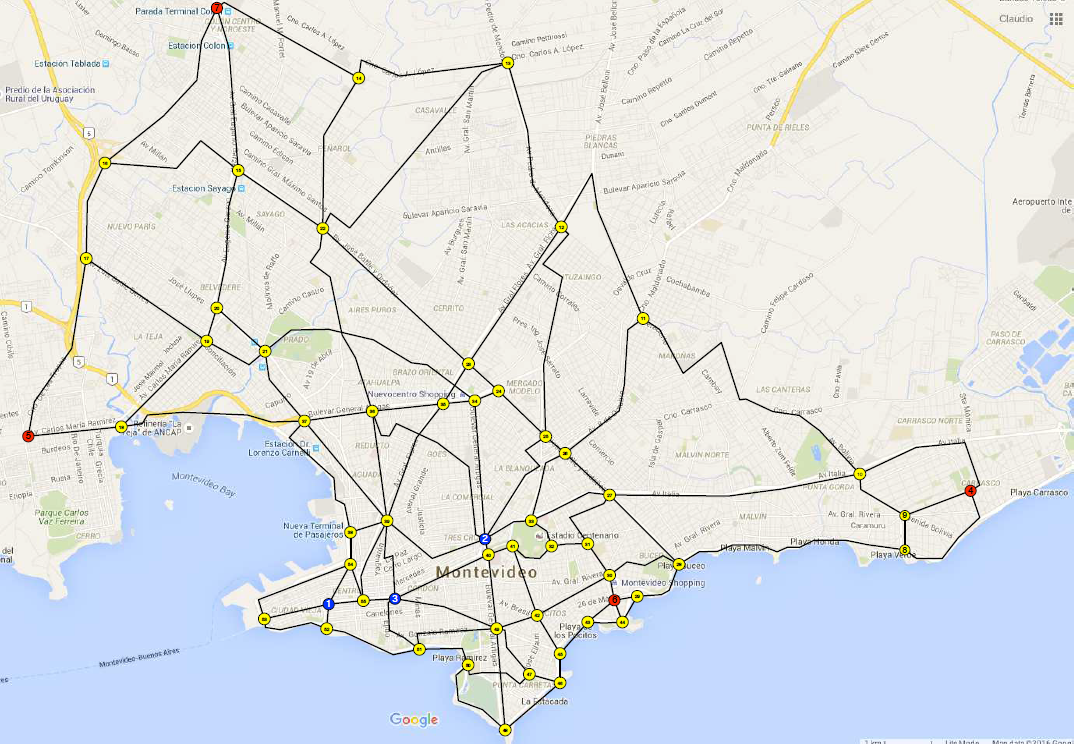
\includegraphics[scale=0.7]{images/FullMap}
\end{align*}

En las siguientes secciones se presentarán los distintos desafíos del obligatorio y las soluciones propuestas.

\section{Parte I}
\subsection{Minimización por costos}
En una primera aproximación el objetivo fue obtener el trazado de costo mínimo para conectar las terminales con los puntos de concentración planteando el problema como uno de programación lineal y considerando las siguientes restricciones:
\begin{itemize}
	\item Que existan dos líneas (caminos) para conectar tanto Cerro, Colón y Carrasco con los nodos del centro y tres líneas para conectar Pocitos con los nodos del centro.
	\item Que ninguno de los tramos del plano fuera utilizado por más de una línea (las estaciones sí pueden ser parte de más de una línea).
\end{itemize}

\subsubsection{Formulación LP}
\begin{equation}
\begin{array}{rrclcl}
\displaystyle \min & \sum_{(i,j) \in E} c_{ij}.x_{ij}  \\
\textrm{s.t.} s& \sum_{j \in S(i)} x_{ij} - \sum_{j \in E(i)} x_{ji} =\begin{cases}
				0 \text{ si i es un nodo interno del camino}\\
				f_{i} \text{ (flujo saliente de i), si i es una terminal}\\
				\end{cases} 
\\
& 0 & \leq x_{ij} & \leq & 1  & \\
\end{array}
\end{equation}

Considerando entonces el costo total mínimo, se obtuvo entonces que este era de 18076, a continuación se muestra la solución obtenida:
\begin{align*}
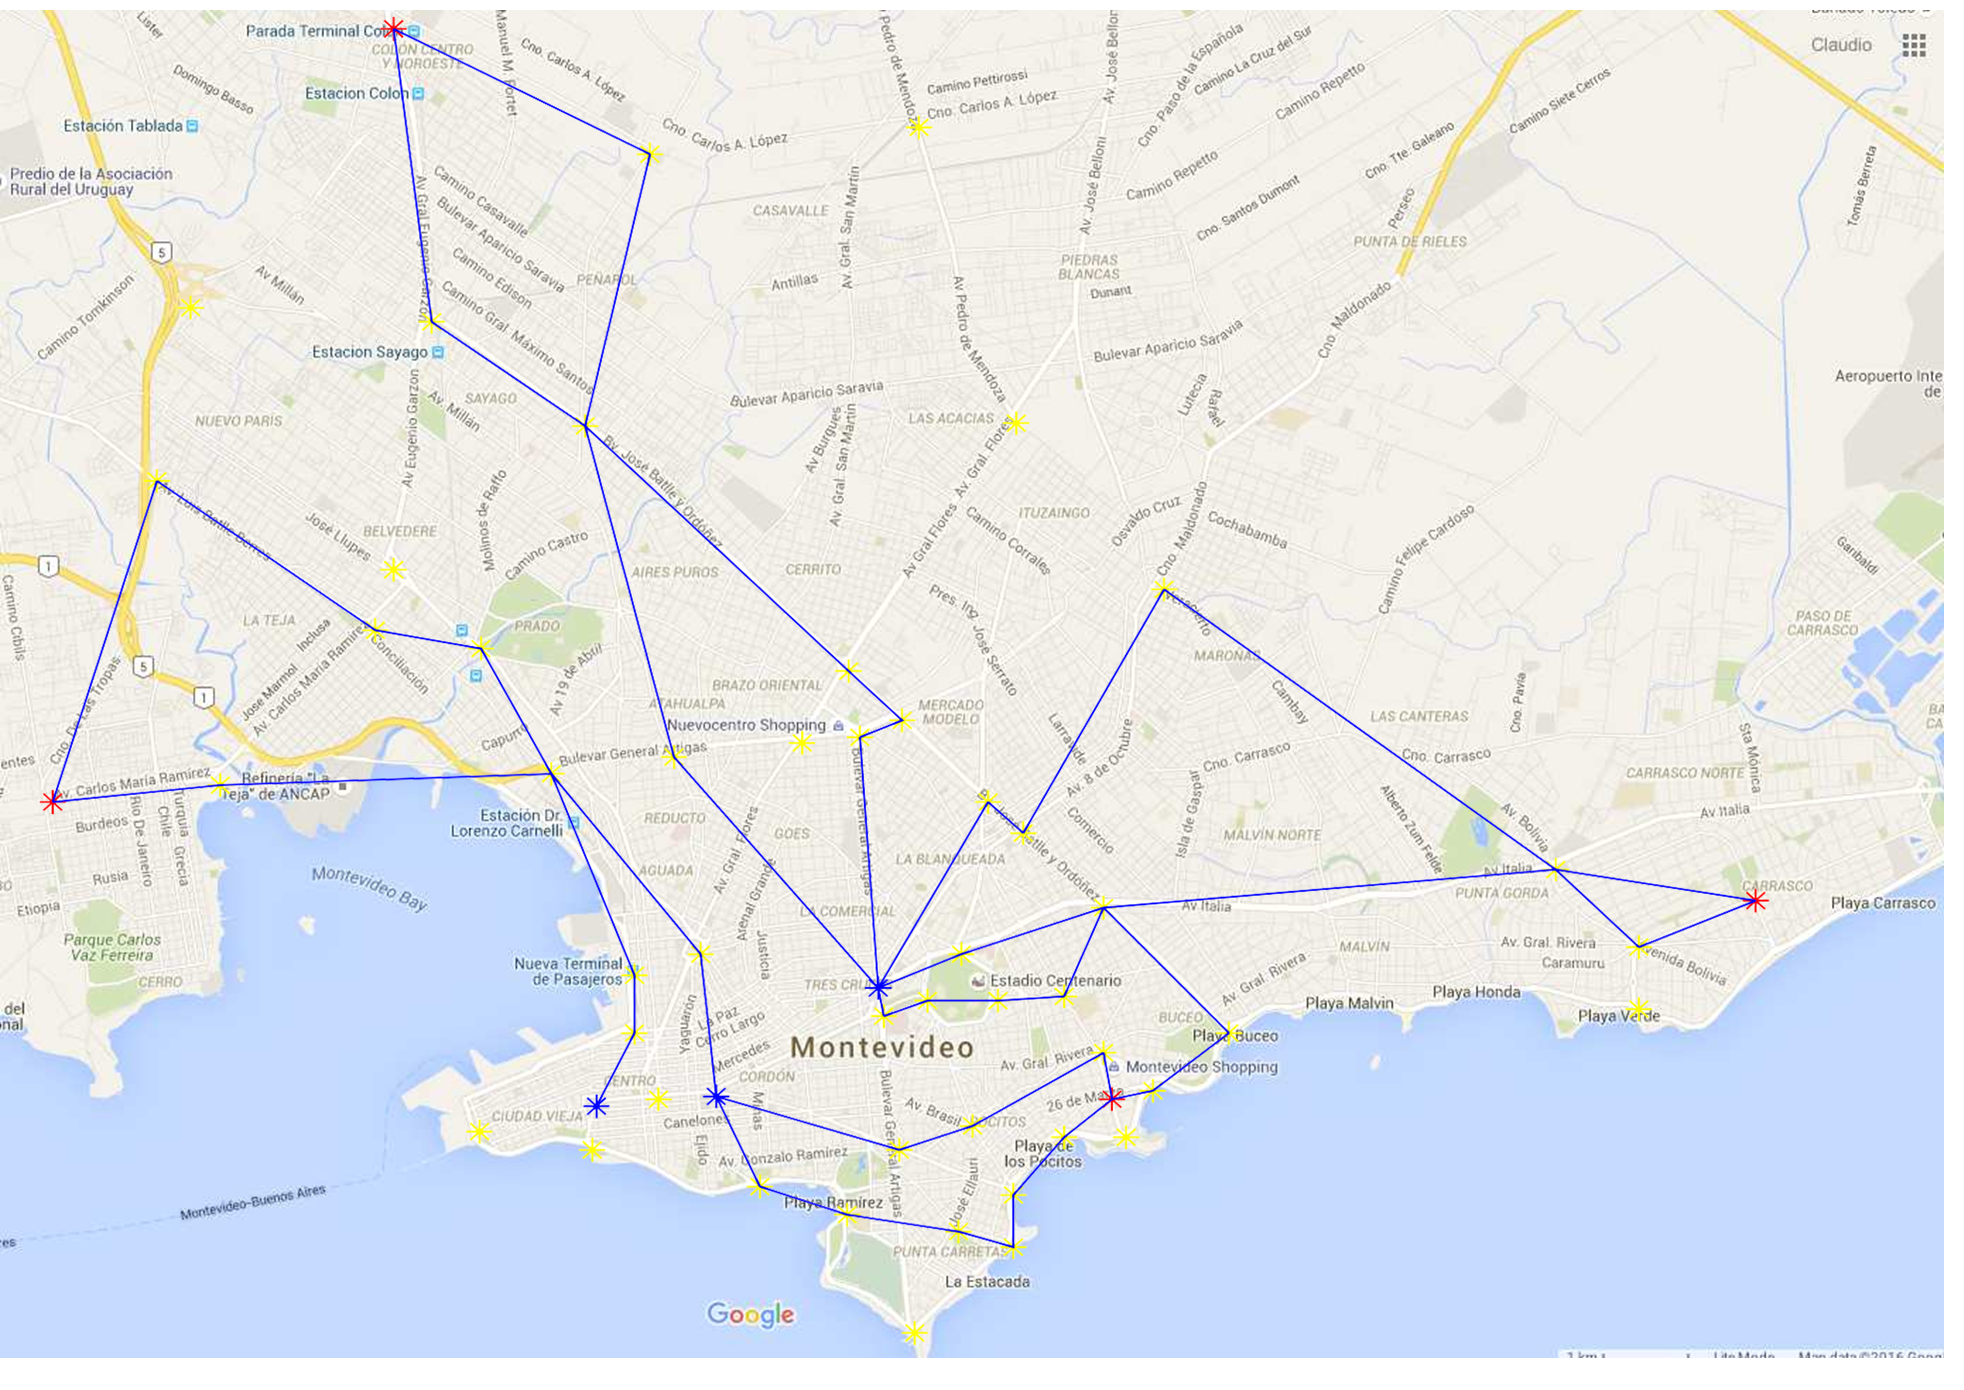
\includegraphics[scale=0.4]{images/f1}
\end{align*}
\newpage
\subsection{Minimización por delay}
Una variante del problema anterior a resolver es la minimización por delay en lugar de costos que resulta análoga a la anterior (considerando la columna de delay en lugar a la de costos).

En este caso el óptimo hallado se corresponde a un delay total de 8512, a continuación se muestra la solución obtenida:
\begin{align*}
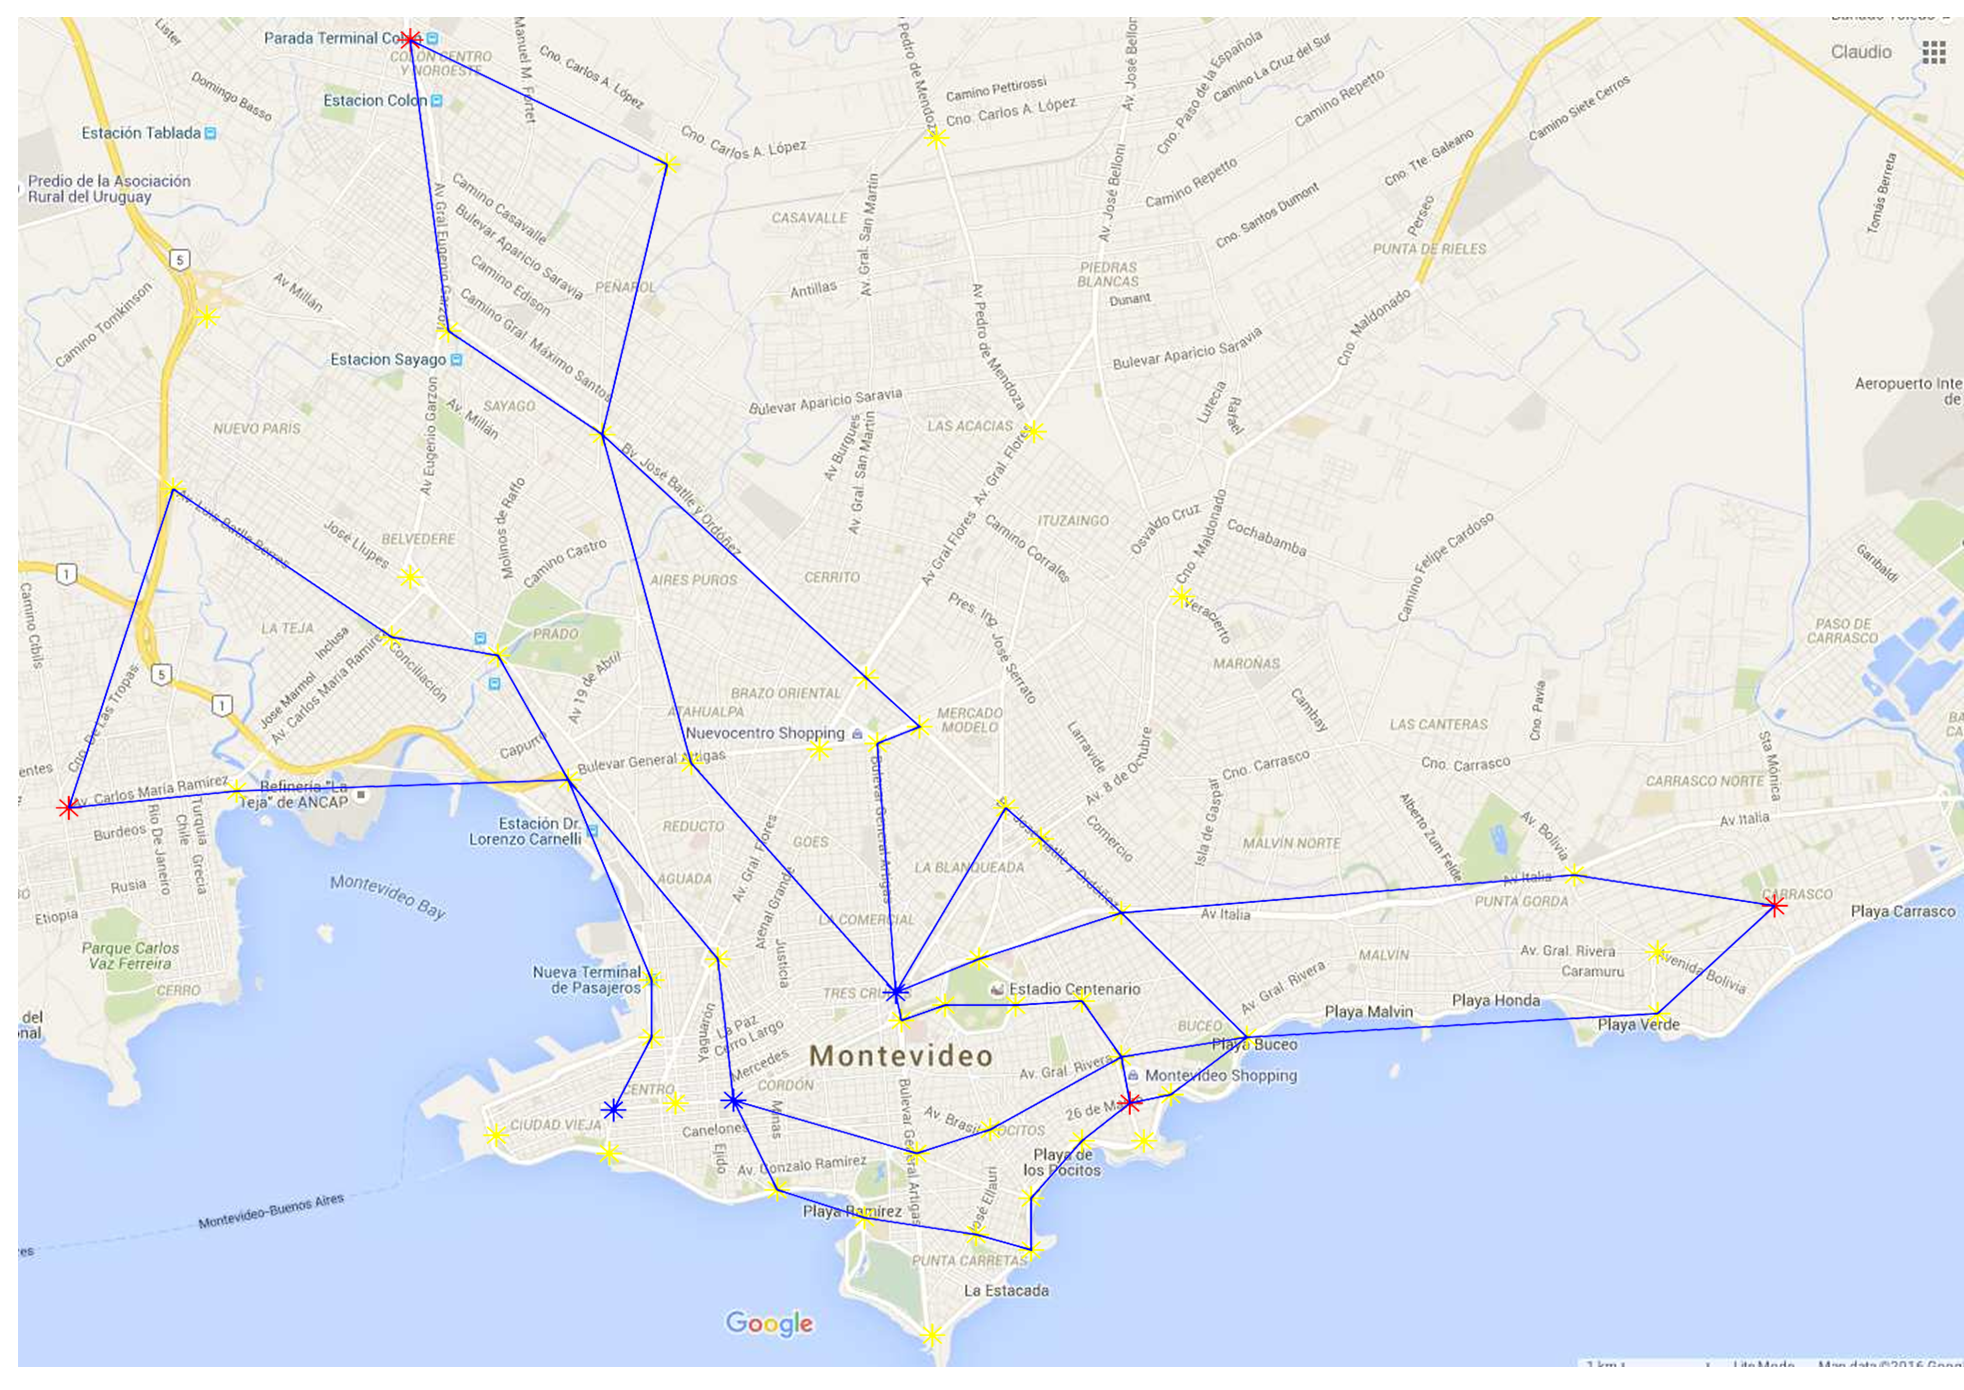
\includegraphics[scale=0.4]{images/f2}
\end{align*}

\subsection{Caminos de costo mínimo}
Como última variante en esta primera parte se calcularon los caminos de costo mínimo, el total fue de 7257 y la solución obtenida se muestra a contnuación:
\begin{align*}
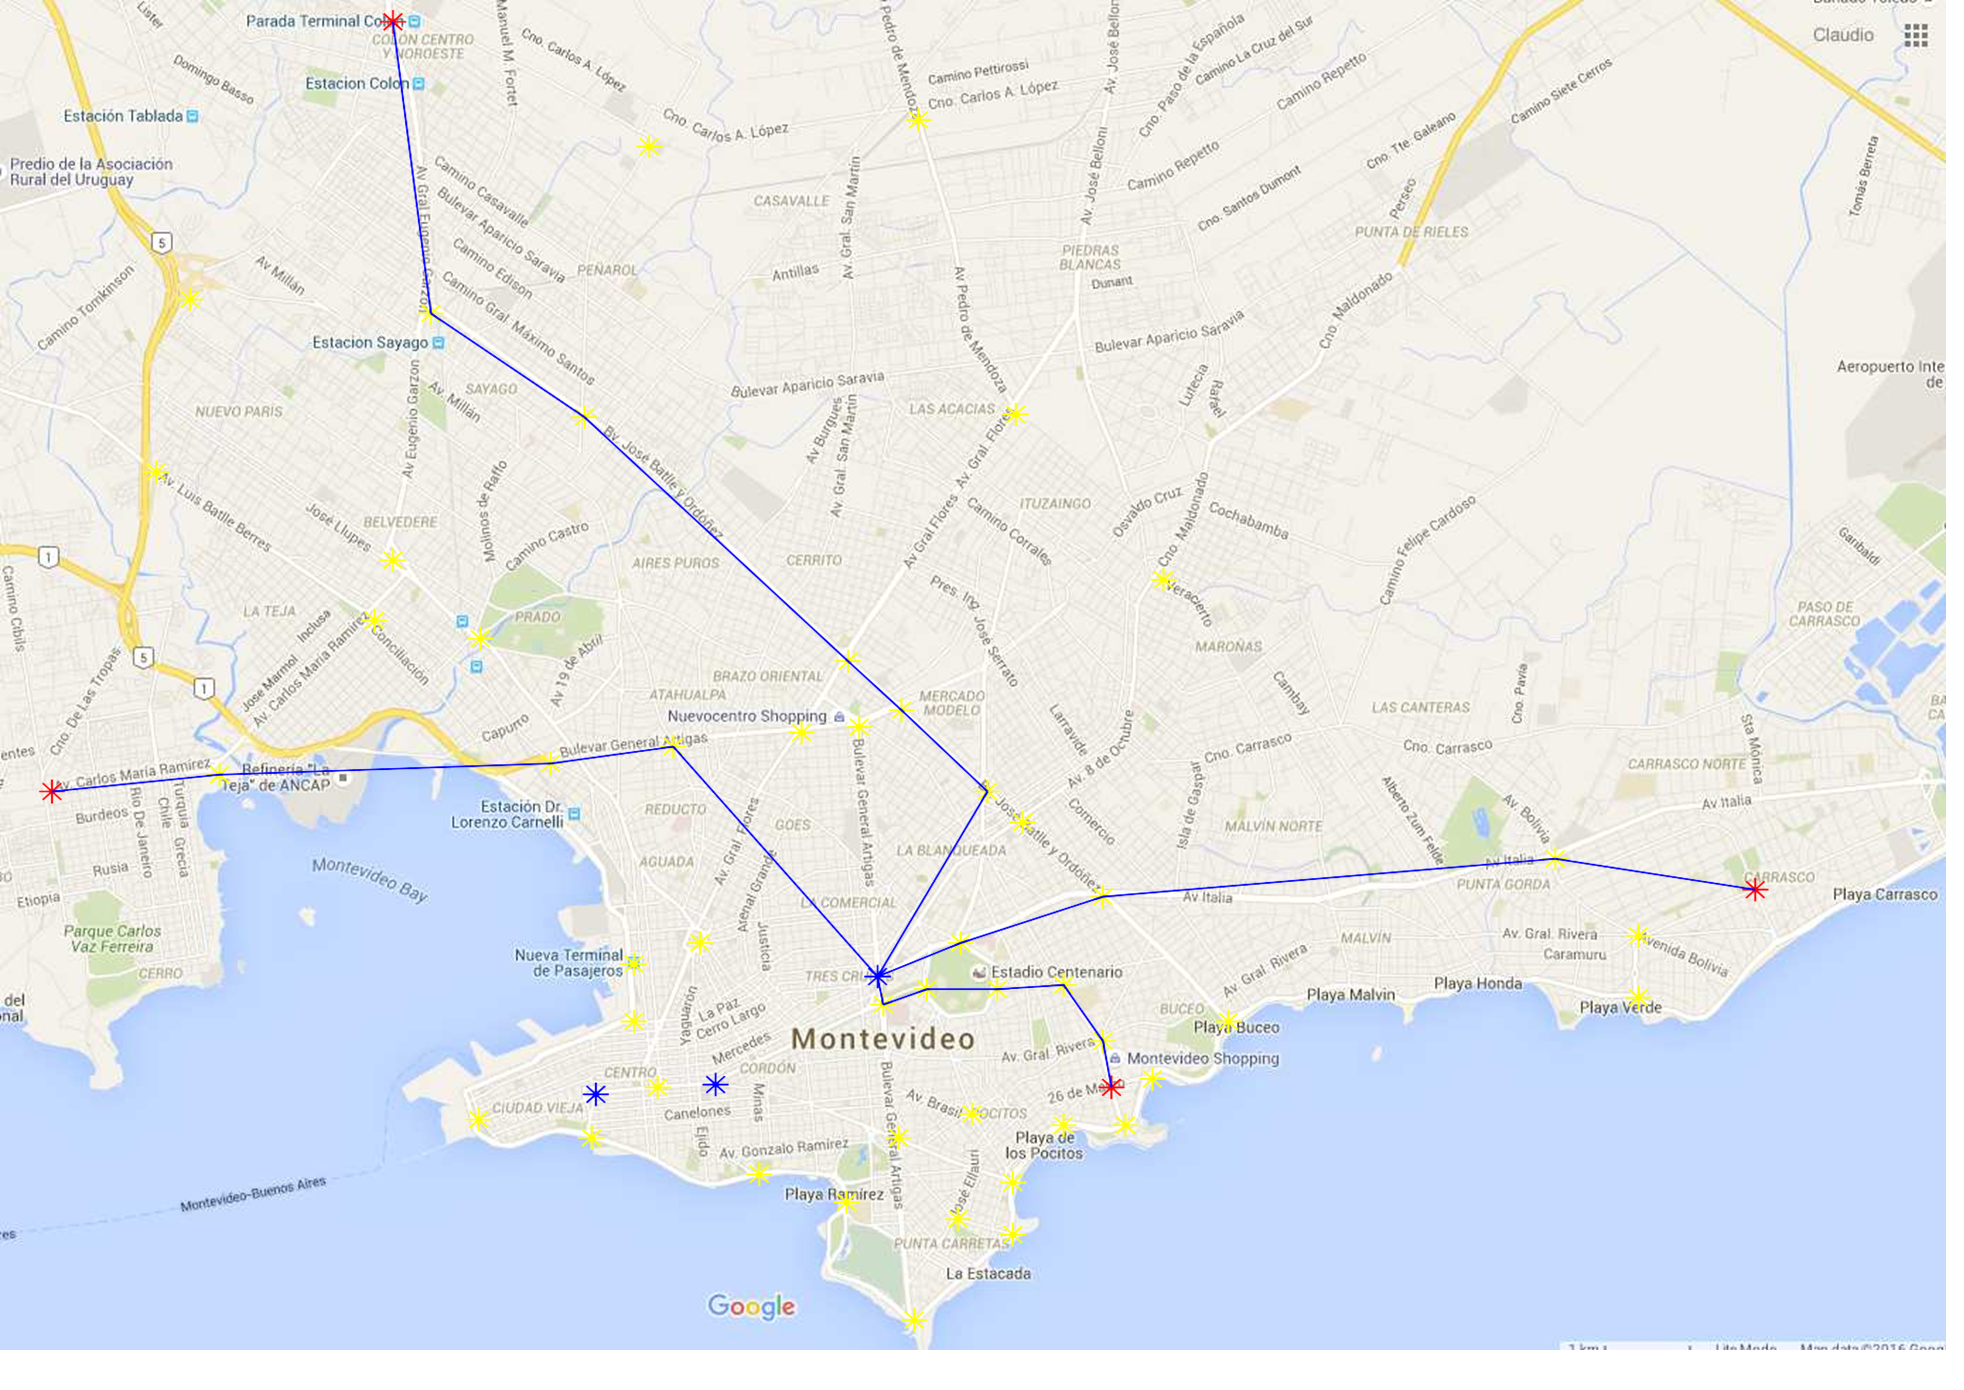
\includegraphics[scale=0.4]{images/f3}
\end{align*}
\subsection{Comparación de resultados}
La siguiente tabla consolida las distintas propuestas considerando para cada una el mínimo total y sus respectivos valores en costo/delay.

\begin{table}[h!]
	\centering
	\caption{Resultados}
	\label{table:levels-sequence}
	\begin{tabular}{|l|l|l|} \hline
		Objetivo  &   Costo Total    & Delay Total   \\
		\hline
		Total por costos        &  118076    & 8700  \\  
		\hline
		Total por delay     &  182572 & 8512 \\
		\hline
		Único camino por costos  &  7257  & 3513  \\
		\hline
		Único camino por delay    &  7850    & 3229   \\
		\hline
	\end{tabular}
\end{table}

En cualquier caso la complejidad del problema es polinomial dado que cuando tenemos múltiples fuentes y sumideros estos problemas se pueden resolver con el algoritmo de Ford-Fulkerson y en el caso de tener caminos únicos alcanza con el algoritmo de dijkstra que es también de orden polinomial.

\section{Parte II}
Bajo las mismas condiciones que la parte anterior se busca ahora la reutilización de tramos entre líneas de distinto origen. Esta nueva versión es una relajación de la anterior dado que la incluye (las soluciones factibles de la parte anterior seguirán siendo factibles en esta versión del problema).
Naturalmente, dado que el objetivo continúa siendo la minimización por costos, al poder reutilizar tramos entre líneas de distinto origen el mínimo encontrado es similar a un ciclo en donde una de las líneas toma el camino más corto mientras que la otra toma el opuesto por lo que el delay se dispara respecto a los encontrados en la versión anterior.

\subsection{Formulación MIP}
COMENTAR EL ENFOQUE CON EL QUE SE RESOLVIÑO ESTA PARTE

\subsection{Resultados}
QUEDA IMAGEN Y COMPARATIVO DE RESULTADOS POR DELAY Y COSTOS EN AMBAS SOLUCIONES DE ESTA PARTE.
\section{Parte III}
El KnapSack Problem (KSP) puede verse como un problema de optimización en el que se busca maximizar la ganancia de artículos incluídos en la mochila considerando que los pesos respectivos de los objetos no superen un umbral total. La siguiente es una formulación LP de este problema:
\begin{equation}
\begin{array}{rrclcl}
\displaystyle \max & \sum_{i=0}^{n} v_ix_i  \\
\textrm{s.t.} & \sum_{i=0}^{n} p_ix_i & \leq & b \\
& 0 \geq x_i & \geq & 1  &, & \forall i \in N \\
\end{array}
\end{equation}

El problema del camino de costo mínimo (CCM) consiste en encontrar un camino de costo mínimo dados dos vértices s y t en un grafo G. En este problema el costo está dado por el peso de la arista pero existen varias variantes a este problema que incluyen restricciones adicionales dando lugar a una familia de problemas que recibe el nombre de Constrained Shortest Path Problems.
Si suponemos que las aristas tienen dos atributos diferentes (peso y costo) y que queremos encontrar el camino de costo mínimo restricto a que los pesos de las aristas del camino no superen un umbral dado tenemos una variante del CCM que resulta ser la instancia más sencilla del problema a resolver en esta parte dado que como mínimo siempre tendremos al menos una fuente y un sumidero.

Por lo tanto, si probamos que esta variante es NP-C el problema de esta parte también será NP-C dado que en todas sus instancias precisaremos resolver al menos una vez un problema que es NP-C.
Cabe notar que al probar la NP-Completitud del problema queda demostrado que este es NP-Hard por definición de NP-Completitud.

Realizaremos la prueba a partir de una reducción del KSP a la variante del CCM descrita anteriormente.

\begin{demo}
	Dada una instancia del KnapSack con artículos en \{1,...,n\}, cada uno de valor $v_{i}$ y peso $p_{i}$, para cada $j=1,...,n$, construiremos un grafo de $n$ nodos de la siguiente forma:
	\begin{align*}
	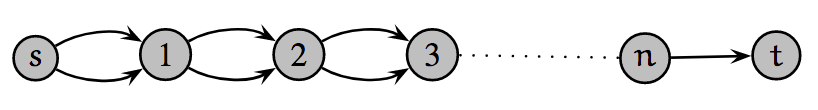
\includegraphics[scale=0.7]{images/grafoDemo}
	\end{align*}
	
	En este grafo de aristas paralelas asociaremos a las superiores las tuplas $(M-v_{j},p_{j})$\footnote{$M = max\{v_{j}: j=1,..,n-1\}$} y $(M,0)$ a las inferiores considerando que en la variante del CCM el costo se corresponde con el primer componente de una tupla y la cantidad máxima de flujo de una arista con la segunda componente.
	
	Luego, podemos ver entonces que si existe un camino de costo mínimo en el grafo que cumpla con las restricciones de flujo encontramos una solución para el KSP y viceversa con lo cual hemos encontrado una reducción y por tanto que la variante de esta parte es un problema NP-C.
		
\end{demo}	

\section{Parte IV}
\subsection{Introducción}
INTRODUCCIÓN DE ALGORITMOS GENETICOS
\subsection{Inicialización}
A partir del problema planteado en la parte I, se construyen soluciones de caminos de costo mínimo desde una fuente hacia las terminales. Estos caminos surgen de perturbar los costos de las aristas y el mismo proceso se aplica para cada una de las fuentes. Luego, para cada conjunto de líneas factible (en términos de su delay) se combinan se agrupan soluciones de cada parte para generar la red.
Experimentalmente se notó que existen al menos 2 caminos de costo mínimo distintos y factibles para cada fuente a los nodos del centro por lo que se obtiene una población inicial de al menos 16 nodos.
\subsection{Selección}
Basada en ranking, todos los individuos sea rankean y la probabilidad de que sean seleccionados es inversamente proporcional a su posición en el ranking. Se seleccionan 2 a reproducirse y el hijo o los hijos se agregan a la población actual mientras que el miembro más débil es descartado. Así con cada iteración.
\subsection{Cruzamiento y mutaciones}
\begin{itemize}
	\item Buscar nodos en común dentro de los individuos y cruzar en ese punto, en principio todos van al mismo pozo así que no habría mayores problemas en cruzar caminos de fuentes distintas y generar diversidad.
	\item Dado un individuo se buscan caminos de fuentes distintas que compartan un nodo y considerando el mínimo de los tramos faltantes a partir del nodo en común se toma ese mínimo y se modifican el resto de los tramos para continuar por el seleccionado. De esta forma se garantiza que los caminos resultantes van a continuar con delay mínimo y mejorando los costos al reutilizar el menor de los tramos a partir del nodo que tenían en común.
	\item Dado un individuo, tomar una línea y borrarla entera para regenerarla con la restricción de que tenga un delay menor o igual.
\end{itemize}






NOTAS:

idea de claudio: ver cuantos podemos crear
construir cosas factibles de la parte 1 minimizando delay, meterle ruido aleatoriamente a los enlacez cambiando lso delays mas menos un porcentaje y genero muchas instancias y luego veo cuales son factibles

fundamentar eleccion de la metaheuristica y presentarla.
 
 
 fundamentar operadores polinomiales sin caer en resolver problemas que son npcompletos, osea mostrar que generar la poblacion es polinomial y que las otras cosas como hacer una mutación es polinomial (si la mutacion implica hacer un CSP entonces no sirve porque estams resolviendo un subproblema que es polinomial)
 
\section{Parte V}

\section{Referencias consultadas}
	\begin{thebibliography}{99}		
		\bibitem{1} Alves Pessoa, et. al. Robust constrained shortest path problems under budgeted uncertainty.
		
		\bibitem{2} Ziegelmann, M. Constrained Shortest Path and Related Problems. Universitat der Saarlandes. \\
		\url{http://scidok.sulb.uni-saarland.de/volltexte/2004/251/pdf/MarkZiegelmann_ProfDrKurtMehlhorn.pdf}
		
		\bibitem{3} Lecture Notes: Solving linear and integer programs using the GNU linear programming kit.  Duke University. \\ \url{https://www.cs.duke.edu/courses/spring08/cps296.2/solvers.pdf}
		
		\bibitem{4} Lecture Notes: Integer Programming, Relaxations and Bounds. Technische Universitat Kaiserslautern. \\
		\url{http://www.mathematik.uni-kl.de/fileadmin/AGs/opt/Lehre/WS1314/IntegerProgramming_WS1314/ip-chapter6.pdf}
		
	\end{thebibliography}
	
\end{document}